The MOD file format is an old music tracker file format originally created for the Commodore Amiga (figure \ref{img-amiga}), a series of computers from the late eighties.
\begin{figure}[H]
	\centering
	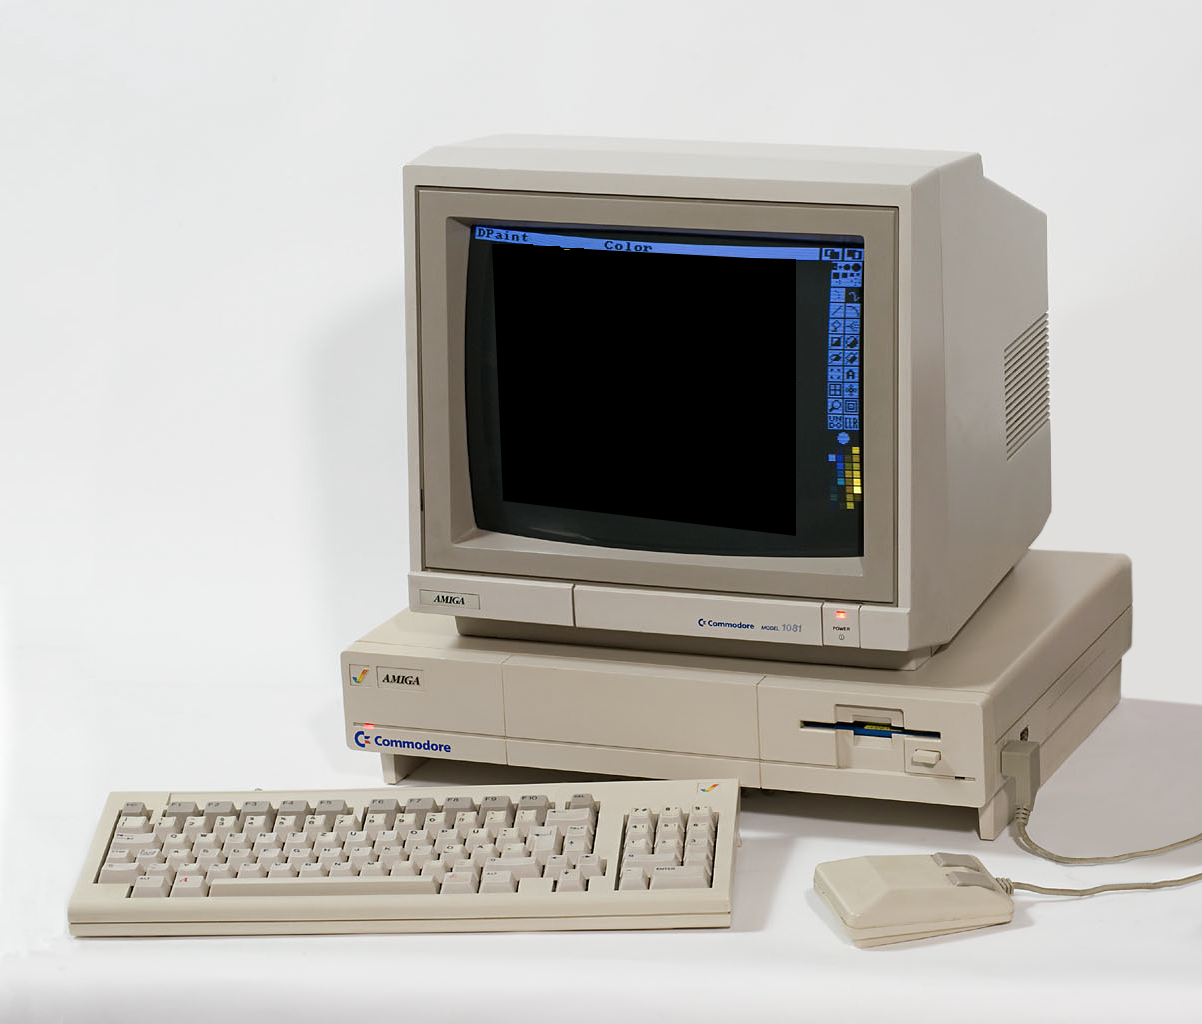
\includegraphics[width=4in]{{images/Amiga.jpg}}
	\caption{The Amiga 1000 (1985), the first Amiga model released. Image courtesy of Kaiiv.}
    \label{img-amiga}
\end{figure}

The file format is tightly optimized for playback on the Amiga's audio hardware, so to understand the inner workings of the MOD file format, one should first know a little about how the Amiga's audio hardware works.

The Amiga's sound chip, called Paula, is capable of powering four simultaneous DMA-driven 8-bit PCM sample sound channels.
Each of these channels can be independently set to different sample frequencies many times per second.
The MOD format exploits this -- it supports 4 simultaneous channels of sample playback, using the frequency modulation to change the pitch of the samples played in the different channels.

Internally, the music in a MOD file is stored as a set of PCM-coded predefined sounds, as well as a large table of note patterns containing information about which sounds should be played at which frequencies and at which time.
The MOD format also includes a large set of musical effects such as tremolo, vibrato, arpeggio, portamento and so on, a subset of which are implemented in the presented solution program.

The MOD file format is not a defined standard, and does therefore not have a formal specification.
The MOD format grew organically from the early Amiga demoscene in the eighties, so many different variants exist -- each with with their own specialities and quirks.
The MOD Player presented in the solution is tailored to read so-called \texttt{M.K.} MODs generated by a MOD creator program (``tracker'') called ProTracker.
These MOD files are called \texttt{M.K.} MODs because they contain the magic number \texttt{M.K.} in the file header.
This is one of the most popular MOD formats, and has become a sort informal standard amongst MOD trackers.

\texttt{M.K.} MODs can have a maximum of 31 bundled PCM-coded sounds, 128 patterns, each with 64 note divisions for each of the four channels, and a a 128 item long list of which patterns should be played in what order.

Figure \ref{img-protracker} shows an image of a MOD file being edited in a tracker program.
Each column represents one channel (called track in ProTracker), and each row represents one of the 64 divisions of a pattern.
The currently played division is traditionally kept vertically centered in the middle of the screen.


\begin{figure}[H]
	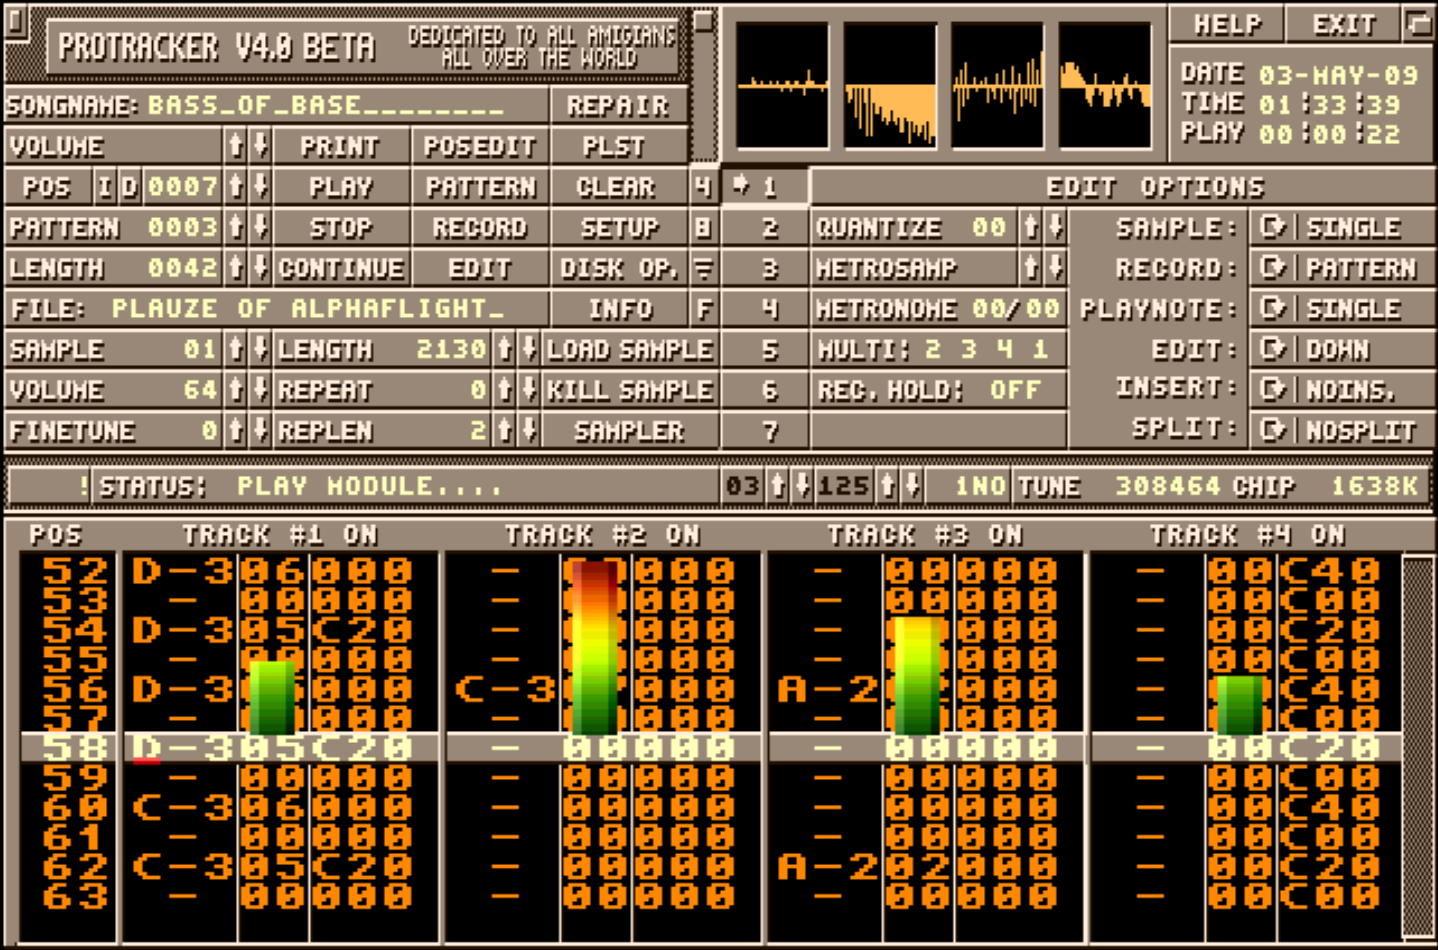
\includegraphics[width = \textwidth]{images/Protracker.png}
	\caption{A four-channel MOD being played in ProTracker. Image courtesy of Alec Graggamoor.}
	\label{img-protracker}
\end{figure}

These four resources do a pretty good job of documenting the MOD file format in detail:
\begin{itemize}
	\item{\url{http://www.mediatel.lu/workshop/audio/fileformat/h_mod.html}}
	\item{\url{http://archive.cs.uu.nl/pub/MIDI/DOC/MOD-info}}
	\item{\url{https://bel.fi/alankila/modguide/}}
	\item{\url{http://16-bits.org/mod/}}
\end{itemize}

\newpage
